\documentclass[10pt,pdf,hyperref={unicode}]{beamer}

\usepackage[normalem]{ulem}
\usepackage{qrcode}
\usepackage{array}
\usepackage[T2A]{fontenc}
\usepackage[utf8]{inputenc}
\usepackage{colortbl}
\usepackage{minted}
\usepackage{listings}
\usepackage{tcolorbox}

\setbeamertemplate{navigation symbols}{}

\usetheme{default}

\usepackage{array}
\newcolumntype{L}[1]{>{\raggedright\let\newline\\\arraybackslash\hspace{0pt}}m{#1}}
\newcolumntype{C}[1]{>{\centering\let\newline\\\arraybackslash\hspace{0pt}}m{#1}}
\newcolumntype{R}[1]{>{\raggedleft\let\newline\\\arraybackslash\hspace{0pt}}m{#1}}

\definecolor{shadecolor}{RGB}{210,210,210}
\newcommand{\asm}[1]{\colorbox{shadecolor}{#1}}

\newcommand{\qrlinkframe}[2]{\begin{frame}{#1}
\center\qrcode[hyperlink,height=75px]{#2}
\end{frame}}

\title{Семинар 14: виртуальная память}
\date{17 марта, 2020}


\begin{document}

\begin{frame}
  \titlepage
\end{frame}

\begin{frame}{Фрагментация памяти}
\begin{itemize}
    \item Для выделения памяти в операционных системах обычно используется два подхода
    \item \textbf{Сегментация} -- память делится на куски разной длины и затем раздаётся
    \item Однако это ведёт к \textbf{фрагментации} -- в какой-то момент может быть ситуация, когда каждый второй байт занят и программа требует половину памяти; несмотря на то, что в реальности 50\% памяти свободно, выделить её невозможно
    \item Второй подход -- \textbf{paging} или \textbf{табличная адресация}
\end{itemize}
\end{frame}

\begin{frame}{Виртуальная память и страничная адресация}
\begin{itemize}
    \item Вся физическая память разделена на \emph{фреймы} — куски размером 4096 байт
    \item Вся виртуальная память аналогично разделена на \emph{страницы}
    \item Трансляцией виртуальной памяти в физическую занимается \emph{memory management unit} (MMU)
\end{itemize}
\end{frame}

\begin{frame}{Page tables}
\begin{itemize}
    \item Специальные структуры, которые хранят отображение виртуальной памяти в физическую
    \item Всего существует $2^{52}$ страниц памяти
    \item Если каждая страница описывается 8 байтами, то такая структура занимает $2^{60}$ байт в памяти
    \item Нужен более экономный способ хранить это отображение
\end{itemize}
\end{frame}

\begin{frame}{Multi-level page tables}
\begin{itemize}
    \item Идея: давайте сделаем таблицы многоуровневыми — сначала поделим всё пространство на части, каждую из этих частей ещё на части итд
    \item Не храня лишние «дыры» мы будем экономить место
    \onslide<2-> \item Под x86-64 используются четырёхуровневые таблицы: P4, P3, P2, P1.
    \onslide<2-> \item Каждая таблица занимает ровно 4096 байт и содержит 512 записей (\emph{PTE = page table entry}) по 8 байт
    \onslide<2-> \item Каждая запись ссылается на индекс в следующей таблице, последняя таблица ссылается на адрес фрейма
\end{itemize}
\end{frame}

\begin{frame}{Что хранится в PTE?}
\begin{itemize}
    \item Индексация следующей таблицы или фрейма не занимает все 8 байт PTE
    \item Кроме неё в PTE есть ещё специальные \emph{флаги страниц}
    \item Например, 1-ый бит отвечает за то, будет ли страница доступна на запись
    \item 63ий -- за то, будет ли процессор исполнять код на этой странице
    \item Также в некоторые биты процессор сам пишет флаги, например, dirty-бит устанавливается всегда, когда происходит запись в страницу
    \item Флаги имеют иерархическую видимость: если в P2 writeable-бит равен 0, а в P4 -- 1, то страница будет доступна на запись
\end{itemize}
\end{frame}

\begin{frame}{Устройство виртуального адреса}
\begin{itemize}
    \item На текущий момент x86-64 позволяет адресовать 48 бит физической памяти
    \item Старшие биты (с 48 по 63) должны быть sign extended копии 47ого бита
    \item Следующие биты (с 38 по 47) адресуют PTE в P4
    \item Биты с 29 по 37 адресуют PTE в P3
    \item Биты с 21 по 28 адресуют PTE в P2
    \item Биты с 12 по 20 адресуют PTE в P1, которая ссылает непосредственно на фрейм
    \item Биты с 0 по 11 адресуют смещение внутри фрейма
\end{itemize}
\end{frame}

\begin{frame}{Устройство виртуального адреса}
\center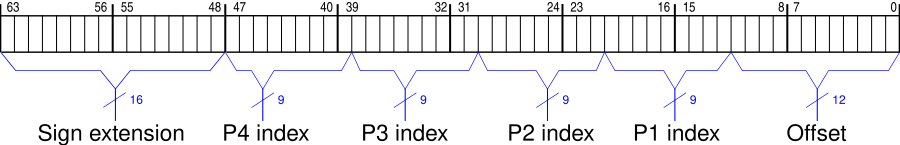
\includegraphics[width=325px]{x86_address_structure.png}
\end{frame}

\begin{frame}{Устройство виртуального адреса}
\center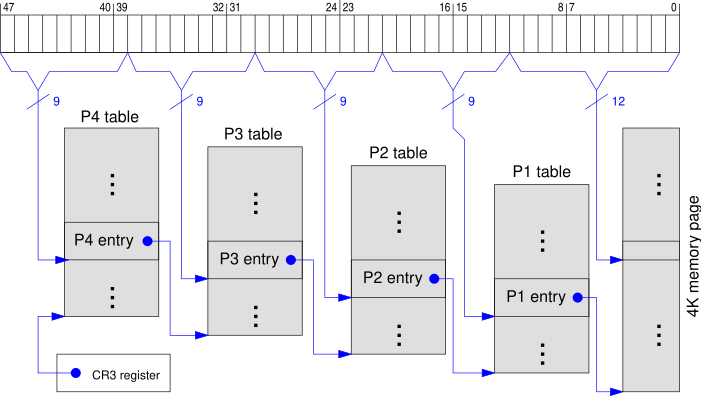
\includegraphics[width=325px]{X86_Paging_64bit.png}
\end{frame}

\begin{frame}{ОС и таблицы страниц}
\begin{itemize}
    \item Операционная система хранит таблицы страниц для каждого процесса
    \item Таблица страниц переключается каждый раз при context switch
    \item Физический адрес текущей P4 хранит специальный регистр CR3 (такие регистры называются \emph{MSR = model specific registers})
    \item В реальности каждое обращение к памяти не вызывает прыжки по таблицам, оно кэшируется в \emph{TLB = translation lookaside buffer}
    \item При context switch TLB полностью сбрасывается
\end{itemize}
\end{frame}

\begin{frame}{Выделение памяти: on-demand paging}
\begin{itemize}
    \item Современные ОС не выделяют всю запрошенную память сразу
    \item Вместо этого используется on-demand paging
    \item Если страницы нет в текущем memory mapping'е, то процессор сгенерирует специальное исключение, называемое \emph{page fault}'ом
    \item Идея состоит в том, чтобы детектировать с помощью page fault'ов реальные обращения к памяти и только тогда её выделять
\end{itemize}
\end{frame}

\begin{frame}{Выделение памяти: minor page}
\begin{itemize}
    \item Кроме самих таблиц страниц ОС обычно хранят свои отображения, запрошенные пользователем
    \item В Linux такие отображения называются \emph{VMA = virtual memory areas}
    \item В ядре они хранятся в КЧ-дереве
    \item Когда пользователь выделяет новый участок виртуальной памяти, ядро создаёт VMA и добавляет его в дерево, но не выделяет ему страницу
    \item Когда происходит первое обращение к любому байту в этой области, MMU видит, что отображения на физическую память нет и выбрасывает page fault
    \item Ядро перехватывает его, видит, что тут должна быть физическая страничка, выделяет её, добавляет в таблицы страниц и возвращает управление в процесс
    \item Это и называется \emph{minor page fault}
\end{itemize}
\end{frame}

\begin{frame}{Выделение памяти: major page faults}
\begin{itemize}
    \item То, что было описано выше справедливо для т.н. \emph{anonymous mappings} -- маппингов, за которыми скрыта только RAM-память, отдельная для каждого процесса
    \item Однако, Linux позволяет производить \emph{file memory mapping}, то есть отображение файла в память по фиксированному адресу — там будет начало файла
    \item Для таких страниц Linux тоже выделяет VMA, но они называются \emph{shared}
    \item Для них тоже используется on-demand paging: при первом обращении генерируется page fault, ядро перехватывает исключение, читает с диска файл и копирует его в память
    \item Это называется \emph{major page fault}
\end{itemize}
\end{frame}

\begin{frame}[fragile]
\frametitle{Интерфейс Linux для работы с VMA: mmap и munmap}
\begin{center}
    \begin{minipage}{0.95\textwidth}
        \begin{minted}[mathescape=true]{c}
#include <sys/mman.h>

void *mmap(void *addr, size_t length, int prot, int flags,
          int fd, off_t offset);
int munmap(void *addr, size_t length);
int mprotect(void *addr, size_t len, int prot);
        \end{minted}
    \end{minipage}
\end{center}
\end{frame}

\begin{frame}{mmap}
\begin{itemize}
    \item mmap выделяет область виртуальной памяти, начиная с адреса \mintinline{c}{addr} длиной \mintinline{c}{lengh} байт
    \item \mintinline{c}{prot} определяют \emph{режим страницы}
    \item \mintinline{c}{flags} определяют \emph{как} будет страница замапплена
    \item \mintinline{c}{fd} определяет какой файл будет стоять за выделенной областью (\mintinline{c}{offset} -- это оффсет файла, чтобы можно было mmap'ить куски)
\end{itemize}
\end{frame}

\begin{frame}{mmap: prot}
\begin{itemize}
    \item \textbf{PROT\_EXEC} -- процессор сможет выполнять код на этой странице
    \item \textbf{PROT\_READ} -- страница будет доступна на чтение
    \item \textbf{PROT\_WRITE} -- страница будет доступна на запись
    \item \textbf{PROT\_NONE} -- к странице никак нельзя будет обратиться
\end{itemize}
\end{frame}

\begin{frame}{mmap: flags}
\begin{itemize}
    \item \textbf{MAP\_ANONYMOUS} -- определяет, что область будет анонимной, \mintinline{c}{fd == -1}
    \item \textbf{MAP\_SHARED} -- определяет, что область будет доступна детям текущего процесса
    \item \textbf{MAP\_FIXED} -- говорит ядру использовать \emph{в точности} адрес \mintinline{c}{addr} или вернуть ошибку
    \item \textbf{MAP\_POPULATE} -- говорит ядру сразу выделить физическую память для этой области
\end{itemize}
\end{frame}

\begin{frame}{Псевдофайлы для контроля расхода памяти}
\begin{itemize}
    \item \mintinline{c}{/proc/<pid>/maps} хранит текущие VMA
    \item \mintinline{c}{/proc/<pid>/status} содержит статус процесса, есть куча информации о памяти
    \item \mintinline{c}{/proc/<pid>/mem} представляет собой память процесса (её можно читать и писать)
    \item \mintinline{c}{/proc/<pid>/map_files} -- директория, хранит список файлов, которые замапленны в процесс
\end{itemize}
\end{frame}

\begin{frame}{Вытеснение страниц и swap}
\begin{itemize}
    \item Если системе не хватает памяти для хранения страниц файлов, она начинает их сбрасывать на диск
    \item Обычно это никак не заметно на приложениях
    \item Однако в условиях hard memory pressure это приводит к странным последствиям: бинарник процесса может из-за этого постоянно вытесняться из памяти и перечитываться обратно
    \item Так можно поступать только с не-анонимными маппингами
    \item Для анонимных страниц обычно выделяется специальная swap-область на диске, куда ОС скидывает редко используемые страницы процессов
\end{itemize}
\end{frame}

\begin{frame}
\center\Huge{Gratias ago!}
\end{frame}


\end{document}
